\subsubsection{Description of the systems}
An S-band system will be used for telemetry and telecommand purposes and for receiving housekeeping data. It is intended to have uplink and downlink capabilities in half-duplex. The model can be found at \cite{SBand} and \cite{SBandDatasheet}.
\begin{figure}[H]
\begin{center}
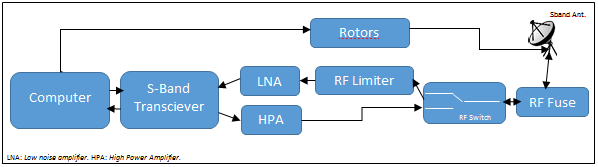
\includegraphics[scale=0.1]{SbandEquip.PNG}
\caption[S-band Equipment]{Equipment needed for S-band communications.}
\label{fig:SbandEquip}
\end{center}
\end{figure}

A X-band system will be used for receiving the data requested by the client from the satellites. It will only have downlink capabilities. The model can be found at \cite{XBand}.
\begin{figure}[H]
\begin{center}
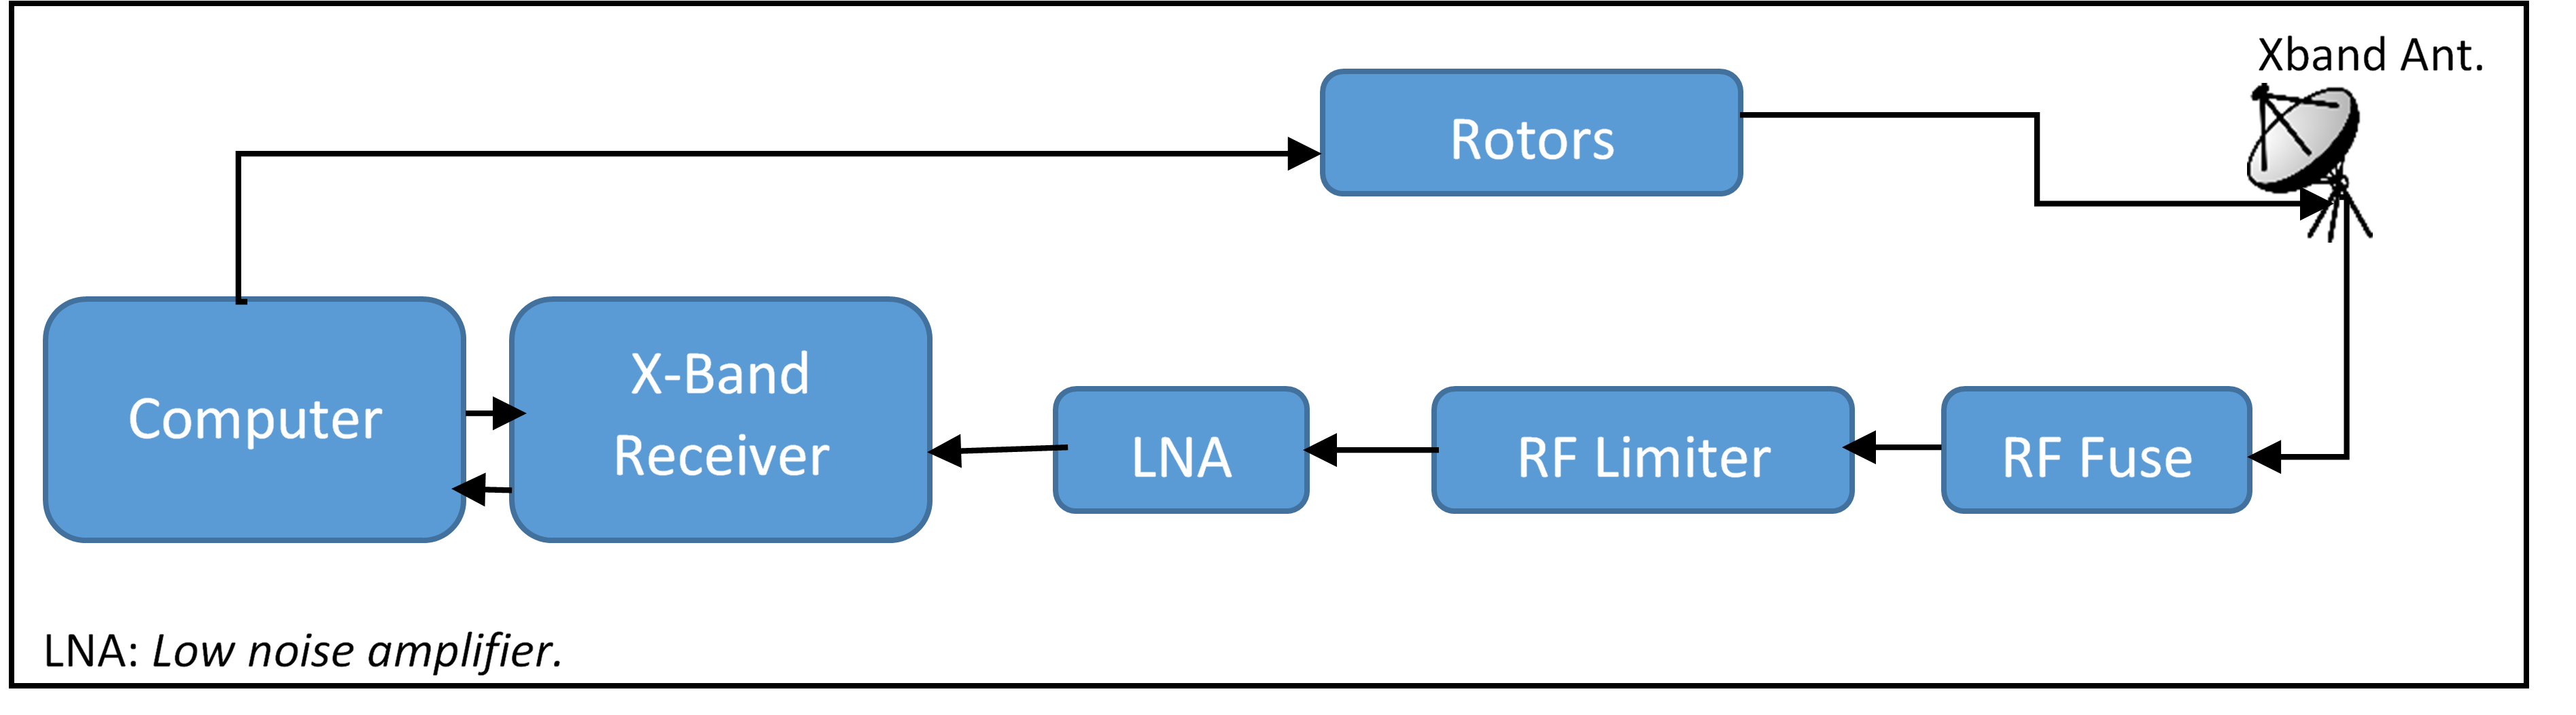
\includegraphics[scale=0.1]{XbandEquip.PNG}
\caption[X-band Equipment]{Equipment needed for X-band communications.}
\label{fig:XbandEquip}
\end{center}
\end{figure}

Because of the time interval in which an antenna will be reorienting itself to point to the next satellite when the current satellite gets out of range, that antenna will not function until it finishes the reorientation. For this reason, two S-band and X-band systems as the ones shown are required for each ground station to be always operative.

\subsubsection{Investment}
In order to calculate the initial investment necessary to build the entire Ground Segment, another economical study must be done. Same as the previous studies, this one can also be found in \cite[Chapter 3, Section 3]{annex3}. The results of said study will be exposed in the following lines:

\begin{itemize}
\item Initial investment of one Ground Station: 356,000\euro
\item Initial investment of the three Ground Stations: 1,070,000\euro
\item Initial investment of the Mission Control Centre: 150,000\euro
\item Initial investment of the whole Ground Segment: 1,220,000\euro
\end{itemize}